\batchmode
\documentclass[letterpaper]{book}
\usepackage{makeidx}
\usepackage{graphicx}
\usepackage{multicol}
\usepackage{float}
\usepackage{listings}
\usepackage{color}
\usepackage{textcomp}
\usepackage{alltt}
\usepackage{times}
\usepackage{ifpdf}
\ifpdf
\usepackage[pdftex,
            pagebackref=true,
            colorlinks=true,
            linkcolor=blue,
            unicode
           ]{hyperref}
\else
\usepackage[ps2pdf,
            pagebackref=true,
            colorlinks=true,
            linkcolor=blue,
            unicode
           ]{hyperref}
\usepackage{pspicture}
\fi
\usepackage[utf8]{inputenc}
\usepackage{doxygen}
\lstset{language=C++,inputencoding=utf8,basicstyle=\footnotesize,breaklines=true,breakatwhitespace=true,tabsize=4,numbers=left }
\makeindex
\setcounter{tocdepth}{3}
\renewcommand{\footrulewidth}{0.4pt}
\begin{document}
\hypersetup{pageanchor=false}
\begin{titlepage}
\vspace*{7cm}
\begin{center}
{\Large Amigo \\[1ex]\large 0.2.0 }\\
\vspace*{1cm}
{\large Generated by Doxygen 1.6.3}\\
\vspace*{0.5cm}
{\small Tue Feb 21 09:26:21 2012}\\
\end{center}
\end{titlepage}
\clearemptydoublepage
\pagenumbering{roman}
\tableofcontents
\clearemptydoublepage
\pagenumbering{arabic}
\hypersetup{pageanchor=true}
\chapter{Class Index}
\section{Class Hierarchy}
This inheritance list is sorted roughly, but not completely, alphabetically:\begin{DoxyCompactList}
\item \contentsline{section}{com::diag::amigo::Display}{\pageref{structcom_1_1diag_1_1amigo_1_1Display}}{}
\begin{DoxyCompactList}
\item \contentsline{section}{Mock}{\pageref{classMock}}{}
\end{DoxyCompactList}
\item \contentsline{section}{com::diag::amigo::LC100Base}{\pageref{classcom_1_1diag_1_1amigo_1_1LC100Base}}{}
\begin{DoxyCompactList}
\item \contentsline{section}{com::diag::amigo::LC100$<$ \_\-COLS\_\-, \_\-ROWS\_\- $>$}{\pageref{classcom_1_1diag_1_1amigo_1_1LC100}}{}
\end{DoxyCompactList}
\end{DoxyCompactList}

\chapter{Class Index}
\section{Class List}
Here are the classes, structs, unions and interfaces with brief descriptions:\begin{DoxyCompactList}
\item\contentsline{section}{\hyperlink{structcom_1_1diag_1_1amigo_1_1Display}{com::diag::amigo::Display} (This pure (abstract) class defines the interface that the \hyperlink{classcom_1_1diag_1_1amigo_1_1LC100}{LC100} software expects to be implemented by any display that it uses )}{\pageref{structcom_1_1diag_1_1amigo_1_1Display}}{}
\item\contentsline{section}{\hyperlink{classcom_1_1diag_1_1amigo_1_1LC100}{com::diag::amigo::LC100$<$ \_\-COLS\_\-, \_\-ROWS\_\- $>$} (This is the derived (sub) class for the \hyperlink{classcom_1_1diag_1_1amigo_1_1LC100}{LC100} software that contains the actual data structures whose sizes depend on the actual size of the display )}{\pageref{classcom_1_1diag_1_1amigo_1_1LC100}}{}
\item\contentsline{section}{\hyperlink{classcom_1_1diag_1_1amigo_1_1LC100Base}{com::diag::amigo::LC100Base} (This is the common base (super) class for the \hyperlink{classcom_1_1diag_1_1amigo_1_1LC100}{LC100} software that does all of the heavy lifting for any \hyperlink{classcom_1_1diag_1_1amigo_1_1LC100}{LC100} template instantiation regardless of the display dimensions )}{\pageref{classcom_1_1diag_1_1amigo_1_1LC100Base}}{}
\item\contentsline{section}{\hyperlink{classMock}{Mock} (This is a mock display that merely traces itself on the serial output and implements the movement keys used by the visual editor (vi) )}{\pageref{classMock}}{}
\end{DoxyCompactList}

\chapter{File Index}
\section{File List}
Here is a list of all documented files with brief descriptions:\begin{DoxyCompactList}
\item\contentsline{section}{\hyperlink{LC100_8cpp}{LC100.cpp} (Copyright 2012 Digital Aggregates Corporation, Colorado, USA\par
 Licensed under the terms in \hyperlink{README_8h}{README.h}\par
 Chip Overclock mailto:\href{mailto:coverclock@diag.com}{\tt coverclock@diag.com}\par
 \href{http://www.diag.com/navigation/downloads/Amigo.html}{\tt http://www.diag.com/navigation/downloads/Amigo.html}\par
 )}{\pageref{LC100_8cpp}}{}
\item\contentsline{section}{\hyperlink{LC100_8h}{LC100.h} (Copyright 2012 Digital Aggregates Corporation, Colorado, USA\par
 Licensed under the terms in \hyperlink{README_8h}{README.h}\par
 Chip Overclock mailto:\href{mailto:coverclock@diag.com}{\tt coverclock@diag.com}\par
 \href{http://www.diag.com/navigation/downloads/Amigo.html}{\tt http://www.diag.com/navigation/downloads/Amigo.html}\par
 )}{\pageref{LC100_8h}}{}
\item\contentsline{section}{\hyperlink{README_8h}{README.h} (This is the README for this project )}{\pageref{README_8h}}{}
\item\contentsline{section}{\hyperlink{TinyTerminal_8ino}{TinyTerminal.ino} (Copyright 2012 Digital Aggregates Corporation, Colorado, USA\par
 Licensed under the terms in \hyperlink{README_8h}{README.h}\par
 Chip Overclock mailto:\href{mailto:coverclock@diag.com}{\tt coverclock@diag.com}\par
 \href{http://www.diag.com/navigation/downloads/Amigo.html}{\tt http://www.diag.com/navigation/downloads/Amigo.html}\par
 )}{\pageref{TinyTerminal_8ino}}{}
\end{DoxyCompactList}

\chapter{Class Documentation}
\hypertarget{structcom_1_1diag_1_1amigo_1_1Display}{
\section{com::diag::amigo::Display Struct Reference}
\label{structcom_1_1diag_1_1amigo_1_1Display}\index{com::diag::amigo::Display@{com::diag::amigo::Display}}
}


This pure (abstract) class defines the interface that the \hyperlink{classcom_1_1diag_1_1amigo_1_1LC100}{LC100} software expects to be implemented by any display that it uses.  




{\ttfamily \#include $<$LC100.h$>$}

Inheritance diagram for com::diag::amigo::Display:\begin{figure}[H]
\begin{center}
\leavevmode
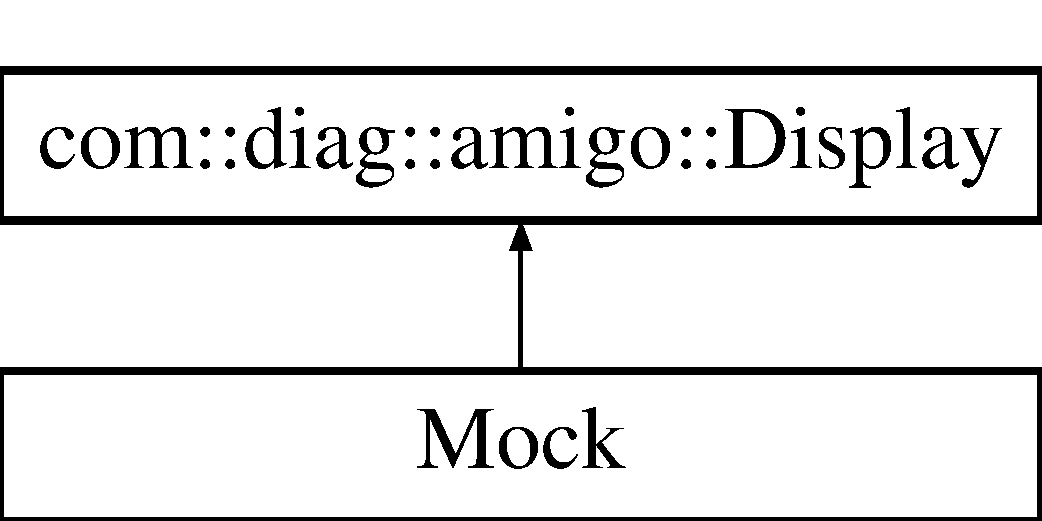
\includegraphics[height=2cm]{structcom_1_1diag_1_1amigo_1_1Display}
\end{center}
\end{figure}
\subsection*{Public Types}
\begin{DoxyCompactItemize}
\item 
enum \hyperlink{structcom_1_1diag_1_1amigo_1_1Display_a57e9915682f8aeb77066171c97c58288}{Read} 
\end{DoxyCompactItemize}
\subsection*{Public Member Functions}
\begin{DoxyCompactItemize}
\item 
virtual void \hyperlink{structcom_1_1diag_1_1amigo_1_1Display_aaa68462ae2314243a31fd7532d51c911}{begin} (byte cols, byte rows)=0
\item 
\hypertarget{structcom_1_1diag_1_1amigo_1_1Display_a8aab5bf6b0cc0183d3b592240c42e6f3}{
virtual void \hyperlink{structcom_1_1diag_1_1amigo_1_1Display_a8aab5bf6b0cc0183d3b592240c42e6f3}{home} ()=0}
\label{structcom_1_1diag_1_1amigo_1_1Display_a8aab5bf6b0cc0183d3b592240c42e6f3}

\item 
\hypertarget{structcom_1_1diag_1_1amigo_1_1Display_abe7e1d0bee831b27c20baa105e7c3b4a}{
virtual void \hyperlink{structcom_1_1diag_1_1amigo_1_1Display_abe7e1d0bee831b27c20baa105e7c3b4a}{clear} ()=0}
\label{structcom_1_1diag_1_1amigo_1_1Display_abe7e1d0bee831b27c20baa105e7c3b4a}

\item 
virtual void \hyperlink{structcom_1_1diag_1_1amigo_1_1Display_ab5356a375bc24de2be5ce1b05bd9fd56}{setCursor} (byte col, byte row)=0
\item 
virtual size\_\-t \hyperlink{structcom_1_1diag_1_1amigo_1_1Display_a4fa3864436e551a42135fbbd3bcb1a3f}{write} (uint8\_\-t ch)=0
\item 
virtual \hyperlink{structcom_1_1diag_1_1amigo_1_1Display_a57e9915682f8aeb77066171c97c58288}{Read} \hyperlink{structcom_1_1diag_1_1amigo_1_1Display_ac630c8e1bbb3ce3091e6db01e1c383e7}{read} ()=0
\end{DoxyCompactItemize}


\subsection{Detailed Description}
This pure (abstract) class defines the interface that the \hyperlink{classcom_1_1diag_1_1amigo_1_1LC100}{LC100} software expects to be implemented by any display that it uses. 

Definition at line 24 of file LC100.h.



\subsection{Member Function Documentation}
\hypertarget{structcom_1_1diag_1_1amigo_1_1Display_aaa68462ae2314243a31fd7532d51c911}{
\index{com::diag::amigo::Display@{com::diag::amigo::Display}!begin@{begin}}
\index{begin@{begin}!com::diag::amigo::Display@{com::diag::amigo::Display}}
\subsubsection[{begin}]{\setlength{\rightskip}{0pt plus 5cm}virtual void com::diag::amigo::Display::begin (byte {\em cols}, \/  byte {\em rows})\hspace{0.3cm}{\ttfamily  \mbox{[}pure virtual\mbox{]}}}}
\label{structcom_1_1diag_1_1amigo_1_1Display_aaa68462ae2314243a31fd7532d51c911}


Initialize. 

This needs to be done only once. 
\begin{DoxyParams}{Parameters}
\item[{\em cols}]is the number of columns in this display. \item[{\em rows}]is the number of rows in this display. \end{DoxyParams}


Implemented in \hyperlink{classMock_abe7c9964a0b81f8bef519f744b700ea5}{Mock}.



Referenced by com::diag::amigo::LC100Base::begin().

\hypertarget{structcom_1_1diag_1_1amigo_1_1Display_ac630c8e1bbb3ce3091e6db01e1c383e7}{
\index{com::diag::amigo::Display@{com::diag::amigo::Display}!read@{read}}
\index{read@{read}!com::diag::amigo::Display@{com::diag::amigo::Display}}
\subsubsection[{read}]{\setlength{\rightskip}{0pt plus 5cm}virtual {\bf Read} com::diag::amigo::Display::read ()\hspace{0.3cm}{\ttfamily  \mbox{[}pure virtual\mbox{]}}}}
\label{structcom_1_1diag_1_1amigo_1_1Display_ac630c8e1bbb3ce3091e6db01e1c383e7}


Read the joystick. 

The returned value will be an enumerated value indicating movement left, down, up, or right, a select indication, or no input. \begin{DoxyReturn}{Returns}
an enumerated value. 
\end{DoxyReturn}


Implemented in \hyperlink{classMock_a0fb6d589bee9e919766e1bb17076351c}{Mock}.



Referenced by com::diag::amigo::LC100Base::read().

\hypertarget{structcom_1_1diag_1_1amigo_1_1Display_ab5356a375bc24de2be5ce1b05bd9fd56}{
\index{com::diag::amigo::Display@{com::diag::amigo::Display}!setCursor@{setCursor}}
\index{setCursor@{setCursor}!com::diag::amigo::Display@{com::diag::amigo::Display}}
\subsubsection[{setCursor}]{\setlength{\rightskip}{0pt plus 5cm}virtual void com::diag::amigo::Display::setCursor (byte {\em col}, \/  byte {\em row})\hspace{0.3cm}{\ttfamily  \mbox{[}pure virtual\mbox{]}}}}
\label{structcom_1_1diag_1_1amigo_1_1Display_ab5356a375bc24de2be5ce1b05bd9fd56}


Place the cursor at the specified position. 

The column and row coordinates are taken modulo of the actual display dimensions. 
\begin{DoxyParams}{Parameters}
\item[{\em col}]is the zero-\/based column number. \item[{\em row}]is the zero-\/based row number. \end{DoxyParams}


Implemented in \hyperlink{classMock_a5545e824f824b147221b61355cabbd5b}{Mock}.



Referenced by com::diag::amigo::LC100Base::down(), com::diag::amigo::LC100Base::setCursor(), and com::diag::amigo::LC100Base::up().

\hypertarget{structcom_1_1diag_1_1amigo_1_1Display_a4fa3864436e551a42135fbbd3bcb1a3f}{
\index{com::diag::amigo::Display@{com::diag::amigo::Display}!write@{write}}
\index{write@{write}!com::diag::amigo::Display@{com::diag::amigo::Display}}
\subsubsection[{write}]{\setlength{\rightskip}{0pt plus 5cm}virtual size\_\-t com::diag::amigo::Display::write (uint8\_\-t {\em ch})\hspace{0.3cm}{\ttfamily  \mbox{[}pure virtual\mbox{]}}}}
\label{structcom_1_1diag_1_1amigo_1_1Display_a4fa3864436e551a42135fbbd3bcb1a3f}


Write a character to the display. 

The signed value that is returned will typically be one, but can be zero if the specified character was somehow invalid, or negative if an error writing the character occurred. 
\begin{DoxyParams}{Parameters}
\item[{\em ch}]is the character that is written to the display. \end{DoxyParams}
\begin{DoxyReturn}{Returns}
the number of characters written. 
\end{DoxyReturn}


Implemented in \hyperlink{classMock_ac3d7b857783204d996cd3e0a147a4ac5}{Mock}.



Referenced by com::diag::amigo::LC100Base::down(), com::diag::amigo::LC100Base::emit(), and com::diag::amigo::LC100Base::up().



The documentation for this struct was generated from the following file:\begin{DoxyCompactItemize}
\item 
\hyperlink{LC100_8h}{LC100.h}\end{DoxyCompactItemize}

\hypertarget{classcom_1_1diag_1_1amigo_1_1LC100}{
\section{com::diag::amigo::LC100$<$ \_\-COLS\_\-, \_\-ROWS\_\- $>$ Class Template Reference}
\label{classcom_1_1diag_1_1amigo_1_1LC100}\index{com::diag::amigo::LC100@{com::diag::amigo::LC100}}
}


This is the derived (sub) class for the \hyperlink{classcom_1_1diag_1_1amigo_1_1LC100}{LC100} software that contains the actual data structures whose sizes depend on the actual size of the display.  




{\ttfamily \#include $<$LC100.h$>$}

Inheritance diagram for com::diag::amigo::LC100$<$ \_\-COLS\_\-, \_\-ROWS\_\- $>$:\begin{figure}[H]
\begin{center}
\leavevmode
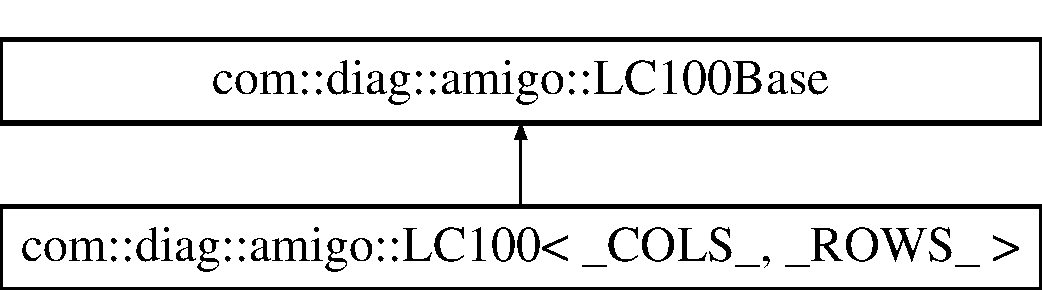
\includegraphics[height=2cm]{classcom_1_1diag_1_1amigo_1_1LC100}
\end{center}
\end{figure}
\subsection*{Public Types}
\begin{DoxyCompactItemize}
\item 
enum \hyperlink{classcom_1_1diag_1_1amigo_1_1LC100Base_af03411f6b7c62f305335952ea45b3d51}{Ascii} 
\end{DoxyCompactItemize}
\subsection*{Public Member Functions}
\begin{DoxyCompactItemize}
\item 
\hyperlink{classcom_1_1diag_1_1amigo_1_1LC100_a731566b8debd903b62c873851641534f}{LC100} (\hyperlink{structcom_1_1diag_1_1amigo_1_1Display}{Display} \&\hyperlink{TinyTerminal_8ino_aa69ecd18e38aaa6c48d94adc9f91f0ef}{display}, boolean sample=false, boolean debug=false, int ms=0)
\item 
\hypertarget{classcom_1_1diag_1_1amigo_1_1LC100_adf882a468cb6b06439927ed426929396}{
virtual \hyperlink{classcom_1_1diag_1_1amigo_1_1LC100_adf882a468cb6b06439927ed426929396}{$\sim$LC100} ()}
\label{classcom_1_1diag_1_1amigo_1_1LC100_adf882a468cb6b06439927ed426929396}

\item 
void \hyperlink{classcom_1_1diag_1_1amigo_1_1LC100Base_a3cf988ae645ac743c6b5cafa2748e30b}{begin} ()
\item 
void \hyperlink{classcom_1_1diag_1_1amigo_1_1LC100Base_aadfb19a306738b52afb990734a412b94}{setCursor} (byte col, byte row)
\item 
\hypertarget{classcom_1_1diag_1_1amigo_1_1LC100Base_aaa8a0afa8ba3d93bc7230f42d794c620}{
void \hyperlink{classcom_1_1diag_1_1amigo_1_1LC100Base_aaa8a0afa8ba3d93bc7230f42d794c620}{home} ()}
\label{classcom_1_1diag_1_1amigo_1_1LC100Base_aaa8a0afa8ba3d93bc7230f42d794c620}

\item 
void \hyperlink{classcom_1_1diag_1_1amigo_1_1LC100Base_af532b82f424d25c8a7b014f16a463abb}{down} ()
\item 
void \hyperlink{classcom_1_1diag_1_1amigo_1_1LC100Base_a836be0f28470396a23a3c28ef835c33d}{up} ()
\item 
void \hyperlink{classcom_1_1diag_1_1amigo_1_1LC100Base_a4a92d06a7c79b66d6fa47581c727f688}{erase} (byte colFrom, byte rowFrom, byte colTo, byte rowTo)
\item 
\hypertarget{classcom_1_1diag_1_1amigo_1_1LC100Base_a91d4bc06663d0d6d9c0e550e3175a55b}{
void \hyperlink{classcom_1_1diag_1_1amigo_1_1LC100Base_a91d4bc06663d0d6d9c0e550e3175a55b}{clear} ()}
\label{classcom_1_1diag_1_1amigo_1_1LC100Base_a91d4bc06663d0d6d9c0e550e3175a55b}

\item 
int \hyperlink{classcom_1_1diag_1_1amigo_1_1LC100Base_a2bbb2cc266ee6a1b9194f12c1ce9c1bf}{read} (char $\ast$buffer)
\item 
size\_\-t \hyperlink{classcom_1_1diag_1_1amigo_1_1LC100Base_aa65643803194c15f83e0204d3523ec7e}{write} (uint8\_\-t ch)
\end{DoxyCompactItemize}
\subsection*{Public Attributes}
\begin{DoxyCompactItemize}
\item 
\hypertarget{classcom_1_1diag_1_1amigo_1_1LC100Base_ae6afb224738640f518910b18b3da5d53}{
const byte \hyperlink{classcom_1_1diag_1_1amigo_1_1LC100Base_ae6afb224738640f518910b18b3da5d53}{COLS}}
\label{classcom_1_1diag_1_1amigo_1_1LC100Base_ae6afb224738640f518910b18b3da5d53}

\item 
\hypertarget{classcom_1_1diag_1_1amigo_1_1LC100Base_a863016b41914b002bd3d4e38486bdf0d}{
const byte \hyperlink{classcom_1_1diag_1_1amigo_1_1LC100Base_a863016b41914b002bd3d4e38486bdf0d}{ROWS}}
\label{classcom_1_1diag_1_1amigo_1_1LC100Base_a863016b41914b002bd3d4e38486bdf0d}

\end{DoxyCompactItemize}
\subsection*{Protected Types}
\begin{DoxyCompactItemize}
\item 
enum \hyperlink{classcom_1_1diag_1_1amigo_1_1LC100Base_a3a022c506359c0a939ed14e4fab577b8}{Constant} 
\item 
enum \hyperlink{classcom_1_1diag_1_1amigo_1_1LC100Base_a13ddf5295a1d05a7d2d939941ba7266e}{State} 
\item 
enum \hyperlink{classcom_1_1diag_1_1amigo_1_1LC100Base_afa1217f48472f7f6758733208ad14125}{Action} 
\end{DoxyCompactItemize}
\subsection*{Protected Member Functions}
\begin{DoxyCompactItemize}
\item 
byte \hyperlink{classcom_1_1diag_1_1amigo_1_1LC100Base_a01be594835cd4bef65fd611bb3e995be}{index} (byte col, byte row)
\item 
byte \hyperlink{classcom_1_1diag_1_1amigo_1_1LC100Base_a2fea6d0b46f653633fdf7677b6ce1f67}{index} (byte row)
\item 
size\_\-t \hyperlink{classcom_1_1diag_1_1amigo_1_1LC100Base_adad20089d65b5744e062a7b02fc14ef6}{emit} (uint8\_\-t ch)
\item 
size\_\-t \hyperlink{classcom_1_1diag_1_1amigo_1_1LC100Base_ae97773781b9decc7a4f6f08eb6ec5162}{frame} (uint8\_\-t ch)
\item 
byte \hyperlink{classcom_1_1diag_1_1amigo_1_1LC100Base_a8e2489e4637dd50cd06e6432c9b50fac}{one} (byte value)
\end{DoxyCompactItemize}


\subsection{Detailed Description}
\subsubsection*{template$<$byte \_\-COLS\_\-, byte \_\-ROWS\_\-$>$ class com::diag::amigo::LC100$<$ \_\-COLS\_\-, \_\-ROWS\_\- $>$}

This is the derived (sub) class for the \hyperlink{classcom_1_1diag_1_1amigo_1_1LC100}{LC100} software that contains the actual data structures whose sizes depend on the actual size of the display. It is templatized so that the display dimensions can be passed as arguments at compile time. 

Definition at line 368 of file LC100.h.



\subsection{Member Enumeration Documentation}
\hypertarget{classcom_1_1diag_1_1amigo_1_1LC100Base_afa1217f48472f7f6758733208ad14125}{
\index{com::diag::amigo::LC100@{com::diag::amigo::LC100}!Action@{Action}}
\index{Action@{Action}!com::diag::amigo::LC100@{com::diag::amigo::LC100}}
\subsubsection[{Action}]{\setlength{\rightskip}{0pt plus 5cm}enum {\bf com::diag::amigo::LC100Base::Action}\hspace{0.3cm}{\ttfamily  \mbox{[}protected, inherited\mbox{]}}}}
\label{classcom_1_1diag_1_1amigo_1_1LC100Base_afa1217f48472f7f6758733208ad14125}


Actions which the push down automaton may execute. 

CONSUMED is the default action. All of the enumerated values are printable, making it easy to trace the PDA as it executes. 

Definition at line 124 of file LC100.h.

\hypertarget{classcom_1_1diag_1_1amigo_1_1LC100Base_a13ddf5295a1d05a7d2d939941ba7266e}{
\index{com::diag::amigo::LC100@{com::diag::amigo::LC100}!State@{State}}
\index{State@{State}!com::diag::amigo::LC100@{com::diag::amigo::LC100}}
\subsubsection[{State}]{\setlength{\rightskip}{0pt plus 5cm}enum {\bf com::diag::amigo::LC100Base::State}\hspace{0.3cm}{\ttfamily  \mbox{[}protected, inherited\mbox{]}}}}
\label{classcom_1_1diag_1_1amigo_1_1LC100Base_a13ddf5295a1d05a7d2d939941ba7266e}


States in which the push down automaton may be. 

DATA is the start state. There is no end state. All of the enumerated values are printable, making it easy to trace the PDA as it executes. 

Definition at line 109 of file LC100.h.



\subsection{Constructor \& Destructor Documentation}
\hypertarget{classcom_1_1diag_1_1amigo_1_1LC100_a731566b8debd903b62c873851641534f}{
\index{com::diag::amigo::LC100@{com::diag::amigo::LC100}!LC100@{LC100}}
\index{LC100@{LC100}!com::diag::amigo::LC100@{com::diag::amigo::LC100}}
\subsubsection[{LC100}]{\setlength{\rightskip}{0pt plus 5cm}template$<$byte \_\-COLS\_\-, byte \_\-ROWS\_\-$>$ {\bf com::diag::amigo::LC100}$<$ \_\-COLS\_\-, \_\-ROWS\_\- $>$::{\bf LC100} ({\bf Display} \& {\em display}, \/  boolean {\em sample} = {\ttfamily false}, \/  boolean {\em debug} = {\ttfamily false}, \/  int {\em ms} = {\ttfamily 0})\hspace{0.3cm}{\ttfamily  \mbox{[}inline\mbox{]}}}}
\label{classcom_1_1diag_1_1amigo_1_1LC100_a731566b8debd903b62c873851641534f}


Ctor. 


\begin{DoxyParams}{Parameters}
\item[{\em display}]refers to the object that implements the \hyperlink{structcom_1_1diag_1_1amigo_1_1Display}{Display} interface. \item[{\em sample}]if true causes the joystick value to be returned continuously as long as a button is pressed; if false, the joystick value is returned intermittently when the button is released. \item[{\em debug}]enables debug output if debugging was compiled in. \item[{\em ms}]is the number of milliseconds to delay between each individual update of the display, which can make debugging a lot easier. \end{DoxyParams}


Definition at line 390 of file LC100.h.



\subsection{Member Function Documentation}
\hypertarget{classcom_1_1diag_1_1amigo_1_1LC100Base_a3cf988ae645ac743c6b5cafa2748e30b}{
\index{com::diag::amigo::LC100@{com::diag::amigo::LC100}!begin@{begin}}
\index{begin@{begin}!com::diag::amigo::LC100@{com::diag::amigo::LC100}}
\subsubsection[{begin}]{\setlength{\rightskip}{0pt plus 5cm}void com::diag::amigo::LC100Base::begin ()\hspace{0.3cm}{\ttfamily  \mbox{[}inherited\mbox{]}}}}
\label{classcom_1_1diag_1_1amigo_1_1LC100Base_a3cf988ae645ac743c6b5cafa2748e30b}


Initialize this object. 

This only needs to be called once. 

Definition at line 724 of file LC100.cpp.



References com::diag::amigo::Display::begin(), com::diag::amigo::LC100Base::clear(), com::diag::amigo::LC100Base::COLS, and com::diag::amigo::LC100Base::ROWS.

\hypertarget{classcom_1_1diag_1_1amigo_1_1LC100Base_af532b82f424d25c8a7b014f16a463abb}{
\index{com::diag::amigo::LC100@{com::diag::amigo::LC100}!down@{down}}
\index{down@{down}!com::diag::amigo::LC100@{com::diag::amigo::LC100}}
\subsubsection[{down}]{\setlength{\rightskip}{0pt plus 5cm}void com::diag::amigo::LC100Base::down ()\hspace{0.3cm}{\ttfamily  \mbox{[}inherited\mbox{]}}}}
\label{classcom_1_1diag_1_1amigo_1_1LC100Base_af532b82f424d25c8a7b014f16a463abb}


Scroll the scroll area down, leaving the cursor placed at a blank line at the top of the scroll area. 

By default, the scroll area is the entire display. 

Definition at line 176 of file LC100.cpp.



References com::diag::amigo::Display::clear(), com::diag::amigo::LC100Base::index(), com::diag::amigo::LC100Base::ROWS, com::diag::amigo::LC100Base::setCursor(), com::diag::amigo::Display::setCursor(), and com::diag::amigo::Display::write().



Referenced by com::diag::amigo::LC100Base::write().

\hypertarget{classcom_1_1diag_1_1amigo_1_1LC100Base_adad20089d65b5744e062a7b02fc14ef6}{
\index{com::diag::amigo::LC100@{com::diag::amigo::LC100}!emit@{emit}}
\index{emit@{emit}!com::diag::amigo::LC100@{com::diag::amigo::LC100}}
\subsubsection[{emit}]{\setlength{\rightskip}{0pt plus 5cm}size\_\-t com::diag::amigo::LC100Base::emit (uint8\_\-t {\em ch})\hspace{0.3cm}{\ttfamily  \mbox{[}protected, inherited\mbox{]}}}}
\label{classcom_1_1diag_1_1amigo_1_1LC100Base_adad20089d65b5744e062a7b02fc14ef6}


Emit a character, which both displays it on the actual display and stores it appropriately in the frame buffer. 

The returned value is the number of characters processed, which is nominally one but may be zero if the character is somehow invalid or negative if an error occurred. 
\begin{DoxyParams}{Parameters}
\item[{\em ch}]is the character to be emitted. \end{DoxyParams}
\begin{DoxyReturn}{Returns}
the number of characters emitted. 
\end{DoxyReturn}


Definition at line 69 of file LC100.cpp.



References com::diag::amigo::LC100Base::COLS, com::diag::amigo::LC100Base::index(), com::diag::amigo::LC100Base::ROWS, and com::diag::amigo::Display::write().



Referenced by com::diag::amigo::LC100Base::erase(), com::diag::amigo::LC100Base::frame(), and com::diag::amigo::LC100Base::write().

\hypertarget{classcom_1_1diag_1_1amigo_1_1LC100Base_a4a92d06a7c79b66d6fa47581c727f688}{
\index{com::diag::amigo::LC100@{com::diag::amigo::LC100}!erase@{erase}}
\index{erase@{erase}!com::diag::amigo::LC100@{com::diag::amigo::LC100}}
\subsubsection[{erase}]{\setlength{\rightskip}{0pt plus 5cm}void com::diag::amigo::LC100Base::erase (byte {\em colFrom}, \/  byte {\em rowFrom}, \/  byte {\em colTo}, \/  byte {\em rowTo})\hspace{0.3cm}{\ttfamily  \mbox{[}inherited\mbox{]}}}}
\label{classcom_1_1diag_1_1amigo_1_1LC100Base_a4a92d06a7c79b66d6fa47581c727f688}


Erase a square bordered by the specified upper left and lower right corners inclusive. 

Erasing is done by writing blanks into the display left to right, top to bottom. The cursor is placed back in its original position. 
\begin{DoxyParams}{Parameters}
\item[{\em colFrom}]is the zero-\/based column of the upper left corner of the erased square. \item[{\em rowFrom}]is the zero-\/based row of the upper left corner of the erased square. \item[{\em colTo}]is the zero-\/based column of the lower right corner of the erased square. \item[{\em rowTo}]is the zero-\/based row of the lower right corner of the erased square. \end{DoxyParams}


Definition at line 109 of file LC100.cpp.



References com::diag::amigo::LC100Base::COLS, com::diag::amigo::LC100Base::emit(), com::diag::amigo::LC100Base::index(), com::diag::amigo::LC100Base::ROWS, and com::diag::amigo::LC100Base::setCursor().



Referenced by com::diag::amigo::LC100Base::frame(), and com::diag::amigo::LC100Base::write().

\hypertarget{classcom_1_1diag_1_1amigo_1_1LC100Base_ae97773781b9decc7a4f6f08eb6ec5162}{
\index{com::diag::amigo::LC100@{com::diag::amigo::LC100}!frame@{frame}}
\index{frame@{frame}!com::diag::amigo::LC100@{com::diag::amigo::LC100}}
\subsubsection[{frame}]{\setlength{\rightskip}{0pt plus 5cm}size\_\-t com::diag::amigo::LC100Base::frame (uint8\_\-t {\em ch})\hspace{0.3cm}{\ttfamily  \mbox{[}protected, inherited\mbox{]}}}}
\label{classcom_1_1diag_1_1amigo_1_1LC100Base_ae97773781b9decc7a4f6f08eb6ec5162}


Frame a character appropriately by dealing with line wrapping (if enabled) and screen scrolling (ditto). 


\begin{DoxyParams}{Parameters}
\item[{\em ch}]is the character to be framed. \end{DoxyParams}
\begin{DoxyReturn}{Returns}
the number of characters framed. 
\end{DoxyReturn}


Definition at line 144 of file LC100.cpp.



References com::diag::amigo::LC100Base::COLS, com::diag::amigo::LC100Base::emit(), com::diag::amigo::LC100Base::erase(), com::diag::amigo::LC100Base::index(), com::diag::amigo::LC100Base::ROWS, com::diag::amigo::LC100Base::setCursor(), and com::diag::amigo::LC100Base::up().



Referenced by com::diag::amigo::LC100Base::write().

\hypertarget{classcom_1_1diag_1_1amigo_1_1LC100Base_a2fea6d0b46f653633fdf7677b6ce1f67}{
\index{com::diag::amigo::LC100@{com::diag::amigo::LC100}!index@{index}}
\index{index@{index}!com::diag::amigo::LC100@{com::diag::amigo::LC100}}
\subsubsection[{index}]{\setlength{\rightskip}{0pt plus 5cm}byte com::diag::amigo::LC100Base::index (byte {\em row})\hspace{0.3cm}{\ttfamily  \mbox{[}protected, inherited\mbox{]}}}}
\label{classcom_1_1diag_1_1amigo_1_1LC100Base_a2fea6d0b46f653633fdf7677b6ce1f67}


Concert a zero-\/based row value into an array index. 


\begin{DoxyParams}{Parameters}
\item[{\em row}]is the zero-\/based row value. \end{DoxyParams}
\begin{DoxyReturn}{Returns}
an array index. 
\end{DoxyReturn}


Definition at line 35 of file LC100.cpp.



References com::diag::amigo::LC100Base::ROWS.

\hypertarget{classcom_1_1diag_1_1amigo_1_1LC100Base_a01be594835cd4bef65fd611bb3e995be}{
\index{com::diag::amigo::LC100@{com::diag::amigo::LC100}!index@{index}}
\index{index@{index}!com::diag::amigo::LC100@{com::diag::amigo::LC100}}
\subsubsection[{index}]{\setlength{\rightskip}{0pt plus 5cm}byte com::diag::amigo::LC100Base::index (byte {\em col}, \/  byte {\em row})\hspace{0.3cm}{\ttfamily  \mbox{[}protected, inherited\mbox{]}}}}
\label{classcom_1_1diag_1_1amigo_1_1LC100Base_a01be594835cd4bef65fd611bb3e995be}


Convert a zero-\/based column and row coordinate into a frame buffer index. 


\begin{DoxyParams}{Parameters}
\item[{\em col}]is the zero-\/based column value. \item[{\em row}]is the zero-\/based row value. \end{DoxyParams}
\begin{DoxyReturn}{Returns}
a frame buffer index. 
\end{DoxyReturn}


Definition at line 39 of file LC100.cpp.



References com::diag::amigo::LC100Base::COLS.



Referenced by com::diag::amigo::LC100Base::down(), com::diag::amigo::LC100Base::emit(), com::diag::amigo::LC100Base::erase(), com::diag::amigo::LC100Base::frame(), com::diag::amigo::LC100Base::up(), and com::diag::amigo::LC100Base::write().

\hypertarget{classcom_1_1diag_1_1amigo_1_1LC100Base_a8e2489e4637dd50cd06e6432c9b50fac}{
\index{com::diag::amigo::LC100@{com::diag::amigo::LC100}!one@{one}}
\index{one@{one}!com::diag::amigo::LC100@{com::diag::amigo::LC100}}
\subsubsection[{one}]{\setlength{\rightskip}{0pt plus 5cm}byte com::diag::amigo::LC100Base::one (byte {\em value})\hspace{0.3cm}{\ttfamily  \mbox{[}protected, inherited\mbox{]}}}}
\label{classcom_1_1diag_1_1amigo_1_1LC100Base_a8e2489e4637dd50cd06e6432c9b50fac}


Convert a one-\/based column or row value into a zero-\/based column or row value. 


\begin{DoxyParams}{Parameters}
\item[{\em value}]is the one-\/based value. \end{DoxyParams}
\begin{DoxyReturn}{Returns}
the zero-\/based value. 
\end{DoxyReturn}


Definition at line 43 of file LC100.cpp.



Referenced by com::diag::amigo::LC100Base::write().

\hypertarget{classcom_1_1diag_1_1amigo_1_1LC100Base_a2bbb2cc266ee6a1b9194f12c1ce9c1bf}{
\index{com::diag::amigo::LC100@{com::diag::amigo::LC100}!read@{read}}
\index{read@{read}!com::diag::amigo::LC100@{com::diag::amigo::LC100}}
\subsubsection[{read}]{\setlength{\rightskip}{0pt plus 5cm}int com::diag::amigo::LC100Base::read (char $\ast$ {\em buffer})\hspace{0.3cm}{\ttfamily  \mbox{[}inherited\mbox{]}}}}
\label{classcom_1_1diag_1_1amigo_1_1LC100Base_a2bbb2cc266ee6a1b9194f12c1ce9c1bf}


Read the current joy stick stimulus into a buffer of at least four bytes in length. 

If the joy stick is indicating movement, the buffer will contain a VT100 (ANSI) arrow escape sequence indicating the direction of movement. The buffer will be nul-\/terminated, allowing it to be written directly to the serial port. Return the number of bytes placed into the buffer, zero indicating that there is no joy stick stimulus at this time. 
\begin{DoxyParams}{Parameters}
\item[{\em buffer}]points to a buffer of at least four bytes in length. \end{DoxyParams}
\begin{DoxyReturn}{Returns}
the number of bytes placed in the buffer. 
\end{DoxyReturn}


Definition at line 667 of file LC100.cpp.



References com::diag::amigo::Display::read().

\hypertarget{classcom_1_1diag_1_1amigo_1_1LC100Base_aadfb19a306738b52afb990734a412b94}{
\index{com::diag::amigo::LC100@{com::diag::amigo::LC100}!setCursor@{setCursor}}
\index{setCursor@{setCursor}!com::diag::amigo::LC100@{com::diag::amigo::LC100}}
\subsubsection[{setCursor}]{\setlength{\rightskip}{0pt plus 5cm}void com::diag::amigo::LC100Base::setCursor (byte {\em col}, \/  byte {\em row})\hspace{0.3cm}{\ttfamily  \mbox{[}inherited\mbox{]}}}}
\label{classcom_1_1diag_1_1amigo_1_1LC100Base_aadfb19a306738b52afb990734a412b94}


Place the cursor at the specified position. 

The column and row coordinates are taken modulo of the actual display dimensions. 
\begin{DoxyParams}{Parameters}
\item[{\em col}]is the zero-\/based column number. \item[{\em row}]is the zero-\/based row number. \end{DoxyParams}


Definition at line 51 of file LC100.cpp.



References com::diag::amigo::LC100Base::COLS, com::diag::amigo::LC100Base::ROWS, and com::diag::amigo::Display::setCursor().



Referenced by com::diag::amigo::LC100Base::clear(), com::diag::amigo::LC100Base::down(), com::diag::amigo::LC100Base::erase(), com::diag::amigo::LC100Base::frame(), com::diag::amigo::LC100Base::up(), and com::diag::amigo::LC100Base::write().

\hypertarget{classcom_1_1diag_1_1amigo_1_1LC100Base_a836be0f28470396a23a3c28ef835c33d}{
\index{com::diag::amigo::LC100@{com::diag::amigo::LC100}!up@{up}}
\index{up@{up}!com::diag::amigo::LC100@{com::diag::amigo::LC100}}
\subsubsection[{up}]{\setlength{\rightskip}{0pt plus 5cm}void com::diag::amigo::LC100Base::up ()\hspace{0.3cm}{\ttfamily  \mbox{[}inherited\mbox{]}}}}
\label{classcom_1_1diag_1_1amigo_1_1LC100Base_a836be0f28470396a23a3c28ef835c33d}


Scroll the scroll area up, leaving the cursor placed at a blank line at the bottom of the scroll area. 

By default, the scroll area is the entire display. 

Definition at line 197 of file LC100.cpp.



References com::diag::amigo::Display::clear(), com::diag::amigo::LC100Base::index(), com::diag::amigo::LC100Base::ROWS, com::diag::amigo::LC100Base::setCursor(), com::diag::amigo::Display::setCursor(), and com::diag::amigo::Display::write().



Referenced by com::diag::amigo::LC100Base::frame(), and com::diag::amigo::LC100Base::write().

\hypertarget{classcom_1_1diag_1_1amigo_1_1LC100Base_aa65643803194c15f83e0204d3523ec7e}{
\index{com::diag::amigo::LC100@{com::diag::amigo::LC100}!write@{write}}
\index{write@{write}!com::diag::amigo::LC100@{com::diag::amigo::LC100}}
\subsubsection[{write}]{\setlength{\rightskip}{0pt plus 5cm}size\_\-t com::diag::amigo::LC100Base::write (uint8\_\-t {\em ch})\hspace{0.3cm}{\ttfamily  \mbox{[}inherited\mbox{]}}}}
\label{classcom_1_1diag_1_1amigo_1_1LC100Base_aa65643803194c15f83e0204d3523ec7e}


Write the current character to the display. 

This character may be part of a VT100 (ANSI) escape sequence, in which case it is not actually written to the display, but will be executed once the complete escape sequence is captured. 
\begin{DoxyParams}{Parameters}
\item[{\em ch}]is the character to be written to the display. \end{DoxyParams}
\begin{DoxyReturn}{Returns}
the number of characters processed, which could be zero if the character is somehow invalid in the context of the current escape sequence, or negative is an error occurred. 
\end{DoxyReturn}


Definition at line 246 of file LC100.cpp.



References com::diag::amigo::LC100Base::clear(), com::diag::amigo::LC100Base::COLS, com::diag::amigo::LC100Base::down(), com::diag::amigo::LC100Base::emit(), com::diag::amigo::LC100Base::erase(), com::diag::amigo::LC100Base::frame(), com::diag::amigo::Display::home(), com::diag::amigo::LC100Base::index(), com::diag::amigo::LC100Base::one(), com::diag::amigo::LC100Base::ROWS, com::diag::amigo::LC100Base::setCursor(), and com::diag::amigo::LC100Base::up().



The documentation for this class was generated from the following file:\begin{DoxyCompactItemize}
\item 
\hyperlink{LC100_8h}{LC100.h}\end{DoxyCompactItemize}

\hypertarget{classcom_1_1diag_1_1amigo_1_1LC100Base}{
\section{com::diag::amigo::LC100Base Class Reference}
\label{classcom_1_1diag_1_1amigo_1_1LC100Base}\index{com::diag::amigo::LC100Base@{com::diag::amigo::LC100Base}}
}


This is the common base (super) class for the \hyperlink{classcom_1_1diag_1_1amigo_1_1LC100}{LC100} software that does all of the heavy lifting for any \hyperlink{classcom_1_1diag_1_1amigo_1_1LC100}{LC100} template instantiation regardless of the display dimensions.  




{\ttfamily \#include $<$LC100.h$>$}

Inheritance diagram for com::diag::amigo::LC100Base:\begin{figure}[H]
\begin{center}
\leavevmode
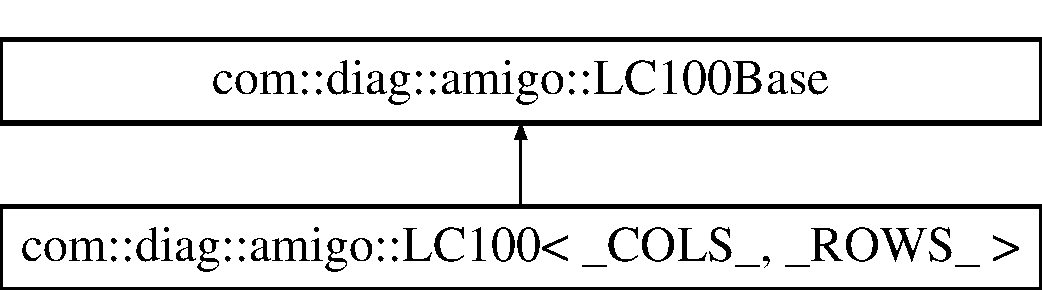
\includegraphics[height=2cm]{classcom_1_1diag_1_1amigo_1_1LC100Base}
\end{center}
\end{figure}
\subsection*{Public Types}
\begin{DoxyCompactItemize}
\item 
enum \hyperlink{classcom_1_1diag_1_1amigo_1_1LC100Base_af03411f6b7c62f305335952ea45b3d51}{Ascii} 
\end{DoxyCompactItemize}
\subsection*{Public Member Functions}
\begin{DoxyCompactItemize}
\item 
\hyperlink{classcom_1_1diag_1_1amigo_1_1LC100Base_a0ae2e5e38c16b74237104acc7a75003c}{LC100Base} (\hyperlink{structcom_1_1diag_1_1amigo_1_1Display}{Display} \&\hyperlink{TinyTerminal_8ino_aa69ecd18e38aaa6c48d94adc9f91f0ef}{display}, byte cols, byte rows, byte $\ast$lineLengthArray, uint8\_\-t $\ast$frameBufferArray, boolean $\ast$tabSettingsArray, boolean sample=false, boolean debug=false, int ms=0)
\item 
\hypertarget{classcom_1_1diag_1_1amigo_1_1LC100Base_ae52a40ef99cf562e26b1f3e2ac072fe5}{
virtual \hyperlink{classcom_1_1diag_1_1amigo_1_1LC100Base_ae52a40ef99cf562e26b1f3e2ac072fe5}{$\sim$LC100Base} ()}
\label{classcom_1_1diag_1_1amigo_1_1LC100Base_ae52a40ef99cf562e26b1f3e2ac072fe5}

\item 
void \hyperlink{classcom_1_1diag_1_1amigo_1_1LC100Base_a3cf988ae645ac743c6b5cafa2748e30b}{begin} ()
\item 
void \hyperlink{classcom_1_1diag_1_1amigo_1_1LC100Base_aadfb19a306738b52afb990734a412b94}{setCursor} (byte col, byte row)
\item 
\hypertarget{classcom_1_1diag_1_1amigo_1_1LC100Base_aaa8a0afa8ba3d93bc7230f42d794c620}{
void \hyperlink{classcom_1_1diag_1_1amigo_1_1LC100Base_aaa8a0afa8ba3d93bc7230f42d794c620}{home} ()}
\label{classcom_1_1diag_1_1amigo_1_1LC100Base_aaa8a0afa8ba3d93bc7230f42d794c620}

\item 
void \hyperlink{classcom_1_1diag_1_1amigo_1_1LC100Base_af532b82f424d25c8a7b014f16a463abb}{down} ()
\item 
void \hyperlink{classcom_1_1diag_1_1amigo_1_1LC100Base_a836be0f28470396a23a3c28ef835c33d}{up} ()
\item 
void \hyperlink{classcom_1_1diag_1_1amigo_1_1LC100Base_a4a92d06a7c79b66d6fa47581c727f688}{erase} (byte colFrom, byte rowFrom, byte colTo, byte rowTo)
\item 
\hypertarget{classcom_1_1diag_1_1amigo_1_1LC100Base_a91d4bc06663d0d6d9c0e550e3175a55b}{
void \hyperlink{classcom_1_1diag_1_1amigo_1_1LC100Base_a91d4bc06663d0d6d9c0e550e3175a55b}{clear} ()}
\label{classcom_1_1diag_1_1amigo_1_1LC100Base_a91d4bc06663d0d6d9c0e550e3175a55b}

\item 
int \hyperlink{classcom_1_1diag_1_1amigo_1_1LC100Base_a2bbb2cc266ee6a1b9194f12c1ce9c1bf}{read} (char $\ast$buffer)
\item 
size\_\-t \hyperlink{classcom_1_1diag_1_1amigo_1_1LC100Base_aa65643803194c15f83e0204d3523ec7e}{write} (uint8\_\-t ch)
\end{DoxyCompactItemize}
\subsection*{Public Attributes}
\begin{DoxyCompactItemize}
\item 
\hypertarget{classcom_1_1diag_1_1amigo_1_1LC100Base_ae6afb224738640f518910b18b3da5d53}{
const byte \hyperlink{classcom_1_1diag_1_1amigo_1_1LC100Base_ae6afb224738640f518910b18b3da5d53}{COLS}}
\label{classcom_1_1diag_1_1amigo_1_1LC100Base_ae6afb224738640f518910b18b3da5d53}

\item 
\hypertarget{classcom_1_1diag_1_1amigo_1_1LC100Base_a863016b41914b002bd3d4e38486bdf0d}{
const byte \hyperlink{classcom_1_1diag_1_1amigo_1_1LC100Base_a863016b41914b002bd3d4e38486bdf0d}{ROWS}}
\label{classcom_1_1diag_1_1amigo_1_1LC100Base_a863016b41914b002bd3d4e38486bdf0d}

\end{DoxyCompactItemize}
\subsection*{Protected Types}
\begin{DoxyCompactItemize}
\item 
enum \hyperlink{classcom_1_1diag_1_1amigo_1_1LC100Base_a3a022c506359c0a939ed14e4fab577b8}{Constant} 
\item 
enum \hyperlink{classcom_1_1diag_1_1amigo_1_1LC100Base_a13ddf5295a1d05a7d2d939941ba7266e}{State} 
\item 
enum \hyperlink{classcom_1_1diag_1_1amigo_1_1LC100Base_afa1217f48472f7f6758733208ad14125}{Action} 
\end{DoxyCompactItemize}
\subsection*{Protected Member Functions}
\begin{DoxyCompactItemize}
\item 
byte \hyperlink{classcom_1_1diag_1_1amigo_1_1LC100Base_a01be594835cd4bef65fd611bb3e995be}{index} (byte col, byte row)
\item 
byte \hyperlink{classcom_1_1diag_1_1amigo_1_1LC100Base_a2fea6d0b46f653633fdf7677b6ce1f67}{index} (byte row)
\item 
size\_\-t \hyperlink{classcom_1_1diag_1_1amigo_1_1LC100Base_adad20089d65b5744e062a7b02fc14ef6}{emit} (uint8\_\-t ch)
\item 
size\_\-t \hyperlink{classcom_1_1diag_1_1amigo_1_1LC100Base_ae97773781b9decc7a4f6f08eb6ec5162}{frame} (uint8\_\-t ch)
\item 
byte \hyperlink{classcom_1_1diag_1_1amigo_1_1LC100Base_a8e2489e4637dd50cd06e6432c9b50fac}{one} (byte value)
\end{DoxyCompactItemize}


\subsection{Detailed Description}
This is the common base (super) class for the \hyperlink{classcom_1_1diag_1_1amigo_1_1LC100}{LC100} software that does all of the heavy lifting for any \hyperlink{classcom_1_1diag_1_1amigo_1_1LC100}{LC100} template instantiation regardless of the display dimensions. It derives from (extends) the Arduino Print class so that any of the usual Print methods can be used by an application. This class is not intended to be used by itself, although there is no reason why you couldn't do so. 

Definition at line 91 of file LC100.h.



\subsection{Member Enumeration Documentation}
\hypertarget{classcom_1_1diag_1_1amigo_1_1LC100Base_afa1217f48472f7f6758733208ad14125}{
\index{com::diag::amigo::LC100Base@{com::diag::amigo::LC100Base}!Action@{Action}}
\index{Action@{Action}!com::diag::amigo::LC100Base@{com::diag::amigo::LC100Base}}
\subsubsection[{Action}]{\setlength{\rightskip}{0pt plus 5cm}enum {\bf com::diag::amigo::LC100Base::Action}\hspace{0.3cm}{\ttfamily  \mbox{[}protected\mbox{]}}}}
\label{classcom_1_1diag_1_1amigo_1_1LC100Base_afa1217f48472f7f6758733208ad14125}


Actions which the push down automaton may execute. 

CONSUMED is the default action. All of the enumerated values are printable, making it easy to trace the PDA as it executes. 

Definition at line 124 of file LC100.h.

\hypertarget{classcom_1_1diag_1_1amigo_1_1LC100Base_a13ddf5295a1d05a7d2d939941ba7266e}{
\index{com::diag::amigo::LC100Base@{com::diag::amigo::LC100Base}!State@{State}}
\index{State@{State}!com::diag::amigo::LC100Base@{com::diag::amigo::LC100Base}}
\subsubsection[{State}]{\setlength{\rightskip}{0pt plus 5cm}enum {\bf com::diag::amigo::LC100Base::State}\hspace{0.3cm}{\ttfamily  \mbox{[}protected\mbox{]}}}}
\label{classcom_1_1diag_1_1amigo_1_1LC100Base_a13ddf5295a1d05a7d2d939941ba7266e}


States in which the push down automaton may be. 

DATA is the start state. There is no end state. All of the enumerated values are printable, making it easy to trace the PDA as it executes. 

Definition at line 109 of file LC100.h.



\subsection{Constructor \& Destructor Documentation}
\hypertarget{classcom_1_1diag_1_1amigo_1_1LC100Base_a0ae2e5e38c16b74237104acc7a75003c}{
\index{com::diag::amigo::LC100Base@{com::diag::amigo::LC100Base}!LC100Base@{LC100Base}}
\index{LC100Base@{LC100Base}!com::diag::amigo::LC100Base@{com::diag::amigo::LC100Base}}
\subsubsection[{LC100Base}]{\setlength{\rightskip}{0pt plus 5cm}com::diag::amigo::LC100Base::LC100Base ({\bf Display} \& {\em display}, \/  byte {\em cols}, \/  byte {\em rows}, \/  byte $\ast$ {\em lineLengthArray}, \/  uint8\_\-t $\ast$ {\em frameBufferArray}, \/  boolean $\ast$ {\em tabSettingsArray}, \/  boolean {\em sample} = {\ttfamily false}, \/  boolean {\em debug} = {\ttfamily false}, \/  int {\em ms} = {\ttfamily 0})\hspace{0.3cm}{\ttfamily  \mbox{[}inline\mbox{]}}}}
\label{classcom_1_1diag_1_1amigo_1_1LC100Base_a0ae2e5e38c16b74237104acc7a75003c}


Ctor. 


\begin{DoxyParams}{Parameters}
\item[{\em display}]refers to the object that implements the \hyperlink{structcom_1_1diag_1_1amigo_1_1Display}{Display} interface. \item[{\em cols}]is the number of columns in the display. \item[{\em rows}]is the number of rows in the display. \item[{\em lineLengthArray}]points to an array of dimension \mbox{[}rows\mbox{]} which will be used to store the length in bytes of the displayed line in each row of the display. \item[{\em frameBufferArray}]points to an array of dimensions \mbox{[}rows\mbox{]}\mbox{[}cols\mbox{]} that is used as a frame buffer to support scrolling. \item[{\em tabSettingsArray}]points to an array of dimension \mbox{[}cols\mbox{]} that is used to keep track of the tab settings for the display. \item[{\em sample}]if true causes the joystick value to be returned continuously as long as a button is pressed; if false, the joystick value is returned intermittently when the button is released. \item[{\em debug}]enables debug output if debugging was compiled in. \item[{\em ms}]is the number of milliseconds to delay between each individual update of the display, which can make debugging a lot easier. \end{DoxyParams}


Definition at line 162 of file LC100.h.



\subsection{Member Function Documentation}
\hypertarget{classcom_1_1diag_1_1amigo_1_1LC100Base_a3cf988ae645ac743c6b5cafa2748e30b}{
\index{com::diag::amigo::LC100Base@{com::diag::amigo::LC100Base}!begin@{begin}}
\index{begin@{begin}!com::diag::amigo::LC100Base@{com::diag::amigo::LC100Base}}
\subsubsection[{begin}]{\setlength{\rightskip}{0pt plus 5cm}void com::diag::amigo::LC100Base::begin ()}}
\label{classcom_1_1diag_1_1amigo_1_1LC100Base_a3cf988ae645ac743c6b5cafa2748e30b}


Initialize this object. 

This only needs to be called once. 

Definition at line 724 of file LC100.cpp.



References com::diag::amigo::Display::begin(), clear(), COLS, and ROWS.

\hypertarget{classcom_1_1diag_1_1amigo_1_1LC100Base_af532b82f424d25c8a7b014f16a463abb}{
\index{com::diag::amigo::LC100Base@{com::diag::amigo::LC100Base}!down@{down}}
\index{down@{down}!com::diag::amigo::LC100Base@{com::diag::amigo::LC100Base}}
\subsubsection[{down}]{\setlength{\rightskip}{0pt plus 5cm}void com::diag::amigo::LC100Base::down ()}}
\label{classcom_1_1diag_1_1amigo_1_1LC100Base_af532b82f424d25c8a7b014f16a463abb}


Scroll the scroll area down, leaving the cursor placed at a blank line at the top of the scroll area. 

By default, the scroll area is the entire display. 

Definition at line 176 of file LC100.cpp.



References com::diag::amigo::Display::clear(), index(), ROWS, setCursor(), com::diag::amigo::Display::setCursor(), and com::diag::amigo::Display::write().



Referenced by write().

\hypertarget{classcom_1_1diag_1_1amigo_1_1LC100Base_adad20089d65b5744e062a7b02fc14ef6}{
\index{com::diag::amigo::LC100Base@{com::diag::amigo::LC100Base}!emit@{emit}}
\index{emit@{emit}!com::diag::amigo::LC100Base@{com::diag::amigo::LC100Base}}
\subsubsection[{emit}]{\setlength{\rightskip}{0pt plus 5cm}size\_\-t com::diag::amigo::LC100Base::emit (uint8\_\-t {\em ch})\hspace{0.3cm}{\ttfamily  \mbox{[}protected\mbox{]}}}}
\label{classcom_1_1diag_1_1amigo_1_1LC100Base_adad20089d65b5744e062a7b02fc14ef6}


Emit a character, which both displays it on the actual display and stores it appropriately in the frame buffer. 

The returned value is the number of characters processed, which is nominally one but may be zero if the character is somehow invalid or negative if an error occurred. 
\begin{DoxyParams}{Parameters}
\item[{\em ch}]is the character to be emitted. \end{DoxyParams}
\begin{DoxyReturn}{Returns}
the number of characters emitted. 
\end{DoxyReturn}


Definition at line 69 of file LC100.cpp.



References COLS, index(), ROWS, and com::diag::amigo::Display::write().



Referenced by erase(), frame(), and write().

\hypertarget{classcom_1_1diag_1_1amigo_1_1LC100Base_a4a92d06a7c79b66d6fa47581c727f688}{
\index{com::diag::amigo::LC100Base@{com::diag::amigo::LC100Base}!erase@{erase}}
\index{erase@{erase}!com::diag::amigo::LC100Base@{com::diag::amigo::LC100Base}}
\subsubsection[{erase}]{\setlength{\rightskip}{0pt plus 5cm}void com::diag::amigo::LC100Base::erase (byte {\em colFrom}, \/  byte {\em rowFrom}, \/  byte {\em colTo}, \/  byte {\em rowTo})}}
\label{classcom_1_1diag_1_1amigo_1_1LC100Base_a4a92d06a7c79b66d6fa47581c727f688}


Erase a square bordered by the specified upper left and lower right corners inclusive. 

Erasing is done by writing blanks into the display left to right, top to bottom. The cursor is placed back in its original position. 
\begin{DoxyParams}{Parameters}
\item[{\em colFrom}]is the zero-\/based column of the upper left corner of the erased square. \item[{\em rowFrom}]is the zero-\/based row of the upper left corner of the erased square. \item[{\em colTo}]is the zero-\/based column of the lower right corner of the erased square. \item[{\em rowTo}]is the zero-\/based row of the lower right corner of the erased square. \end{DoxyParams}


Definition at line 109 of file LC100.cpp.



References COLS, emit(), index(), ROWS, and setCursor().



Referenced by frame(), and write().

\hypertarget{classcom_1_1diag_1_1amigo_1_1LC100Base_ae97773781b9decc7a4f6f08eb6ec5162}{
\index{com::diag::amigo::LC100Base@{com::diag::amigo::LC100Base}!frame@{frame}}
\index{frame@{frame}!com::diag::amigo::LC100Base@{com::diag::amigo::LC100Base}}
\subsubsection[{frame}]{\setlength{\rightskip}{0pt plus 5cm}size\_\-t com::diag::amigo::LC100Base::frame (uint8\_\-t {\em ch})\hspace{0.3cm}{\ttfamily  \mbox{[}protected\mbox{]}}}}
\label{classcom_1_1diag_1_1amigo_1_1LC100Base_ae97773781b9decc7a4f6f08eb6ec5162}


Frame a character appropriately by dealing with line wrapping (if enabled) and screen scrolling (ditto). 


\begin{DoxyParams}{Parameters}
\item[{\em ch}]is the character to be framed. \end{DoxyParams}
\begin{DoxyReturn}{Returns}
the number of characters framed. 
\end{DoxyReturn}


Definition at line 144 of file LC100.cpp.



References COLS, emit(), erase(), index(), ROWS, setCursor(), and up().



Referenced by write().

\hypertarget{classcom_1_1diag_1_1amigo_1_1LC100Base_a2fea6d0b46f653633fdf7677b6ce1f67}{
\index{com::diag::amigo::LC100Base@{com::diag::amigo::LC100Base}!index@{index}}
\index{index@{index}!com::diag::amigo::LC100Base@{com::diag::amigo::LC100Base}}
\subsubsection[{index}]{\setlength{\rightskip}{0pt plus 5cm}byte com::diag::amigo::LC100Base::index (byte {\em row})\hspace{0.3cm}{\ttfamily  \mbox{[}protected\mbox{]}}}}
\label{classcom_1_1diag_1_1amigo_1_1LC100Base_a2fea6d0b46f653633fdf7677b6ce1f67}


Concert a zero-\/based row value into an array index. 


\begin{DoxyParams}{Parameters}
\item[{\em row}]is the zero-\/based row value. \end{DoxyParams}
\begin{DoxyReturn}{Returns}
an array index. 
\end{DoxyReturn}


Definition at line 35 of file LC100.cpp.



References ROWS.

\hypertarget{classcom_1_1diag_1_1amigo_1_1LC100Base_a01be594835cd4bef65fd611bb3e995be}{
\index{com::diag::amigo::LC100Base@{com::diag::amigo::LC100Base}!index@{index}}
\index{index@{index}!com::diag::amigo::LC100Base@{com::diag::amigo::LC100Base}}
\subsubsection[{index}]{\setlength{\rightskip}{0pt plus 5cm}byte com::diag::amigo::LC100Base::index (byte {\em col}, \/  byte {\em row})\hspace{0.3cm}{\ttfamily  \mbox{[}protected\mbox{]}}}}
\label{classcom_1_1diag_1_1amigo_1_1LC100Base_a01be594835cd4bef65fd611bb3e995be}


Convert a zero-\/based column and row coordinate into a frame buffer index. 


\begin{DoxyParams}{Parameters}
\item[{\em col}]is the zero-\/based column value. \item[{\em row}]is the zero-\/based row value. \end{DoxyParams}
\begin{DoxyReturn}{Returns}
a frame buffer index. 
\end{DoxyReturn}


Definition at line 39 of file LC100.cpp.



References COLS.



Referenced by down(), emit(), erase(), frame(), up(), and write().

\hypertarget{classcom_1_1diag_1_1amigo_1_1LC100Base_a8e2489e4637dd50cd06e6432c9b50fac}{
\index{com::diag::amigo::LC100Base@{com::diag::amigo::LC100Base}!one@{one}}
\index{one@{one}!com::diag::amigo::LC100Base@{com::diag::amigo::LC100Base}}
\subsubsection[{one}]{\setlength{\rightskip}{0pt plus 5cm}byte com::diag::amigo::LC100Base::one (byte {\em value})\hspace{0.3cm}{\ttfamily  \mbox{[}protected\mbox{]}}}}
\label{classcom_1_1diag_1_1amigo_1_1LC100Base_a8e2489e4637dd50cd06e6432c9b50fac}


Convert a one-\/based column or row value into a zero-\/based column or row value. 


\begin{DoxyParams}{Parameters}
\item[{\em value}]is the one-\/based value. \end{DoxyParams}
\begin{DoxyReturn}{Returns}
the zero-\/based value. 
\end{DoxyReturn}


Definition at line 43 of file LC100.cpp.



Referenced by write().

\hypertarget{classcom_1_1diag_1_1amigo_1_1LC100Base_a2bbb2cc266ee6a1b9194f12c1ce9c1bf}{
\index{com::diag::amigo::LC100Base@{com::diag::amigo::LC100Base}!read@{read}}
\index{read@{read}!com::diag::amigo::LC100Base@{com::diag::amigo::LC100Base}}
\subsubsection[{read}]{\setlength{\rightskip}{0pt plus 5cm}int com::diag::amigo::LC100Base::read (char $\ast$ {\em buffer})}}
\label{classcom_1_1diag_1_1amigo_1_1LC100Base_a2bbb2cc266ee6a1b9194f12c1ce9c1bf}


Read the current joy stick stimulus into a buffer of at least four bytes in length. 

If the joy stick is indicating movement, the buffer will contain a VT100 (ANSI) arrow escape sequence indicating the direction of movement. The buffer will be nul-\/terminated, allowing it to be written directly to the serial port. Return the number of bytes placed into the buffer, zero indicating that there is no joy stick stimulus at this time. 
\begin{DoxyParams}{Parameters}
\item[{\em buffer}]points to a buffer of at least four bytes in length. \end{DoxyParams}
\begin{DoxyReturn}{Returns}
the number of bytes placed in the buffer. 
\end{DoxyReturn}


Definition at line 667 of file LC100.cpp.



References com::diag::amigo::Display::read().

\hypertarget{classcom_1_1diag_1_1amigo_1_1LC100Base_aadfb19a306738b52afb990734a412b94}{
\index{com::diag::amigo::LC100Base@{com::diag::amigo::LC100Base}!setCursor@{setCursor}}
\index{setCursor@{setCursor}!com::diag::amigo::LC100Base@{com::diag::amigo::LC100Base}}
\subsubsection[{setCursor}]{\setlength{\rightskip}{0pt plus 5cm}void com::diag::amigo::LC100Base::setCursor (byte {\em col}, \/  byte {\em row})}}
\label{classcom_1_1diag_1_1amigo_1_1LC100Base_aadfb19a306738b52afb990734a412b94}


Place the cursor at the specified position. 

The column and row coordinates are taken modulo of the actual display dimensions. 
\begin{DoxyParams}{Parameters}
\item[{\em col}]is the zero-\/based column number. \item[{\em row}]is the zero-\/based row number. \end{DoxyParams}


Definition at line 51 of file LC100.cpp.



References COLS, ROWS, and com::diag::amigo::Display::setCursor().



Referenced by clear(), down(), erase(), frame(), up(), and write().

\hypertarget{classcom_1_1diag_1_1amigo_1_1LC100Base_a836be0f28470396a23a3c28ef835c33d}{
\index{com::diag::amigo::LC100Base@{com::diag::amigo::LC100Base}!up@{up}}
\index{up@{up}!com::diag::amigo::LC100Base@{com::diag::amigo::LC100Base}}
\subsubsection[{up}]{\setlength{\rightskip}{0pt plus 5cm}void com::diag::amigo::LC100Base::up ()}}
\label{classcom_1_1diag_1_1amigo_1_1LC100Base_a836be0f28470396a23a3c28ef835c33d}


Scroll the scroll area up, leaving the cursor placed at a blank line at the bottom of the scroll area. 

By default, the scroll area is the entire display. 

Definition at line 197 of file LC100.cpp.



References com::diag::amigo::Display::clear(), index(), ROWS, setCursor(), com::diag::amigo::Display::setCursor(), and com::diag::amigo::Display::write().



Referenced by frame(), and write().

\hypertarget{classcom_1_1diag_1_1amigo_1_1LC100Base_aa65643803194c15f83e0204d3523ec7e}{
\index{com::diag::amigo::LC100Base@{com::diag::amigo::LC100Base}!write@{write}}
\index{write@{write}!com::diag::amigo::LC100Base@{com::diag::amigo::LC100Base}}
\subsubsection[{write}]{\setlength{\rightskip}{0pt plus 5cm}size\_\-t com::diag::amigo::LC100Base::write (uint8\_\-t {\em ch})}}
\label{classcom_1_1diag_1_1amigo_1_1LC100Base_aa65643803194c15f83e0204d3523ec7e}


Write the current character to the display. 

This character may be part of a VT100 (ANSI) escape sequence, in which case it is not actually written to the display, but will be executed once the complete escape sequence is captured. 
\begin{DoxyParams}{Parameters}
\item[{\em ch}]is the character to be written to the display. \end{DoxyParams}
\begin{DoxyReturn}{Returns}
the number of characters processed, which could be zero if the character is somehow invalid in the context of the current escape sequence, or negative is an error occurred. 
\end{DoxyReturn}


Definition at line 246 of file LC100.cpp.



References clear(), COLS, down(), emit(), erase(), frame(), com::diag::amigo::Display::home(), index(), one(), ROWS, setCursor(), and up().



The documentation for this class was generated from the following files:\begin{DoxyCompactItemize}
\item 
\hyperlink{LC100_8h}{LC100.h}\item 
\hyperlink{LC100_8cpp}{LC100.cpp}\end{DoxyCompactItemize}

\hypertarget{classMock}{
\section{Mock Class Reference}
\label{classMock}\index{Mock@{Mock}}
}


This is a mock display that merely traces itself on the serial output and implements the movement keys used by the visual editor (vi).  


Inheritance diagram for Mock:\begin{figure}[H]
\begin{center}
\leavevmode
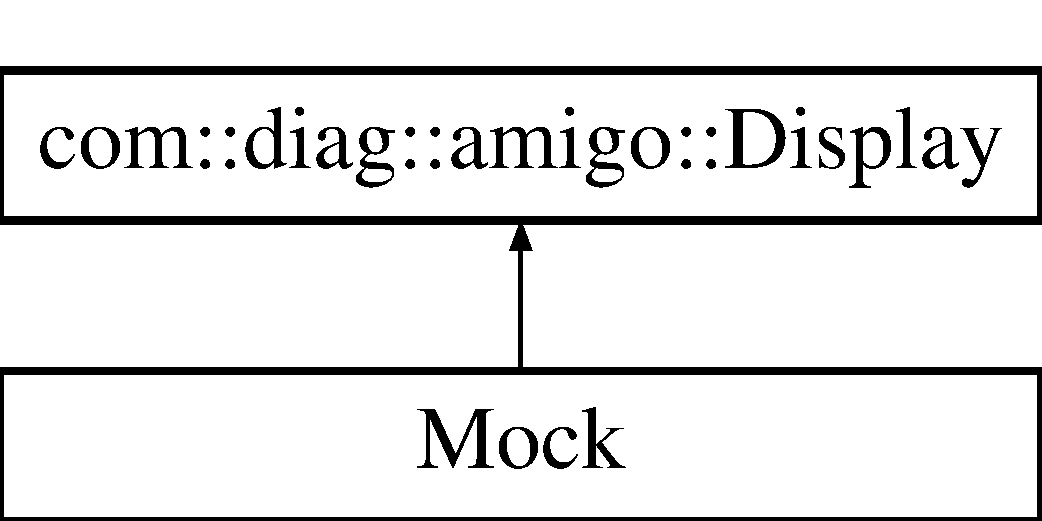
\includegraphics[height=2cm]{classMock}
\end{center}
\end{figure}
\subsection*{Public Types}
\begin{DoxyCompactItemize}
\item 
enum \hyperlink{structcom_1_1diag_1_1amigo_1_1Display_a57e9915682f8aeb77066171c97c58288}{Read} 
\end{DoxyCompactItemize}
\subsection*{Public Member Functions}
\begin{DoxyCompactItemize}
\item 
\hypertarget{classMock_a2b9528f2e7fcf9738201a5ea667c1998}{
\hyperlink{classMock_a2b9528f2e7fcf9738201a5ea667c1998}{Mock} ()}
\label{classMock_a2b9528f2e7fcf9738201a5ea667c1998}

\item 
\hypertarget{classMock_a7b663eff1fa3728433fa84a311833935}{
virtual \hyperlink{classMock_a7b663eff1fa3728433fa84a311833935}{$\sim$Mock} ()}
\label{classMock_a7b663eff1fa3728433fa84a311833935}

\item 
virtual void \hyperlink{classMock_abe7c9964a0b81f8bef519f744b700ea5}{begin} (byte cols, byte rows)
\item 
\hypertarget{classMock_a14f55167d439e1cc71af8a601ce31fa8}{
virtual void \hyperlink{classMock_a14f55167d439e1cc71af8a601ce31fa8}{home} ()}
\label{classMock_a14f55167d439e1cc71af8a601ce31fa8}

\item 
\hypertarget{classMock_a1a7bbca9d17ac5f14e0fc48dd1faab3f}{
virtual void \hyperlink{classMock_a1a7bbca9d17ac5f14e0fc48dd1faab3f}{clear} ()}
\label{classMock_a1a7bbca9d17ac5f14e0fc48dd1faab3f}

\item 
virtual void \hyperlink{classMock_a5545e824f824b147221b61355cabbd5b}{setCursor} (byte col, byte row)
\item 
virtual size\_\-t \hyperlink{classMock_ac3d7b857783204d996cd3e0a147a4ac5}{write} (uint8\_\-t ch)
\item 
virtual \hyperlink{structcom_1_1diag_1_1amigo_1_1Display_a57e9915682f8aeb77066171c97c58288}{Read} \hyperlink{classMock_a0fb6d589bee9e919766e1bb17076351c}{read} ()
\end{DoxyCompactItemize}


\subsection{Detailed Description}
This is a mock display that merely traces itself on the serial output and implements the movement keys used by the visual editor (vi). 

Definition at line 26 of file TinyTerminal.ino.



\subsection{Member Function Documentation}
\hypertarget{classMock_abe7c9964a0b81f8bef519f744b700ea5}{
\index{Mock@{Mock}!begin@{begin}}
\index{begin@{begin}!Mock@{Mock}}
\subsubsection[{begin}]{\setlength{\rightskip}{0pt plus 5cm}virtual void Mock::begin (byte {\em cols}, \/  byte {\em rows})\hspace{0.3cm}{\ttfamily  \mbox{[}inline, virtual\mbox{]}}}}
\label{classMock_abe7c9964a0b81f8bef519f744b700ea5}


Initialize. 

This needs to be done only once. 
\begin{DoxyParams}{Parameters}
\item[{\em cols}]is the number of columns in this display. \item[{\em rows}]is the number of rows in this display. \end{DoxyParams}


Implements \hyperlink{structcom_1_1diag_1_1amigo_1_1Display_aaa68462ae2314243a31fd7532d51c911}{com::diag::amigo::Display}.



Definition at line 47 of file TinyTerminal.ino.

\hypertarget{classMock_a0fb6d589bee9e919766e1bb17076351c}{
\index{Mock@{Mock}!read@{read}}
\index{read@{read}!Mock@{Mock}}
\subsubsection[{read}]{\setlength{\rightskip}{0pt plus 5cm}virtual {\bf Read} Mock::read ()\hspace{0.3cm}{\ttfamily  \mbox{[}inline, virtual\mbox{]}}}}
\label{classMock_a0fb6d589bee9e919766e1bb17076351c}


Read the joystick. 

The returned value will be an enumerated value indicating movement left, down, up, or right, a select indication, or no input. \begin{DoxyReturn}{Returns}
an enumerated value. 
\end{DoxyReturn}


Implements \hyperlink{structcom_1_1diag_1_1amigo_1_1Display_ac630c8e1bbb3ce3091e6db01e1c383e7}{com::diag::amigo::Display}.



Definition at line 106 of file TinyTerminal.ino.

\hypertarget{classMock_a5545e824f824b147221b61355cabbd5b}{
\index{Mock@{Mock}!setCursor@{setCursor}}
\index{setCursor@{setCursor}!Mock@{Mock}}
\subsubsection[{setCursor}]{\setlength{\rightskip}{0pt plus 5cm}virtual void Mock::setCursor (byte {\em col}, \/  byte {\em row})\hspace{0.3cm}{\ttfamily  \mbox{[}inline, virtual\mbox{]}}}}
\label{classMock_a5545e824f824b147221b61355cabbd5b}


Place the cursor at the specified position. 


\begin{DoxyParams}{Parameters}
\item[{\em col}]is the zero-\/based column number. \item[{\em row}]is the zero-\/based row number. \end{DoxyParams}


Implements \hyperlink{structcom_1_1diag_1_1amigo_1_1Display_ab5356a375bc24de2be5ce1b05bd9fd56}{com::diag::amigo::Display}.



Definition at line 73 of file TinyTerminal.ino.

\hypertarget{classMock_ac3d7b857783204d996cd3e0a147a4ac5}{
\index{Mock@{Mock}!write@{write}}
\index{write@{write}!Mock@{Mock}}
\subsubsection[{write}]{\setlength{\rightskip}{0pt plus 5cm}virtual size\_\-t Mock::write (uint8\_\-t {\em ch})\hspace{0.3cm}{\ttfamily  \mbox{[}inline, virtual\mbox{]}}}}
\label{classMock_ac3d7b857783204d996cd3e0a147a4ac5}


Write a character to the display. 

The signed value that is returned will typically be one, but can be zero if the specified character was somehow invalid, or negative if an error writing the character occurred. 
\begin{DoxyParams}{Parameters}
\item[{\em ch}]is the character that is written to the display. \end{DoxyParams}
\begin{DoxyReturn}{Returns}
the number of characters written. 
\end{DoxyReturn}


Implements \hyperlink{structcom_1_1diag_1_1amigo_1_1Display_a4fa3864436e551a42135fbbd3bcb1a3f}{com::diag::amigo::Display}.



Definition at line 87 of file TinyTerminal.ino.



The documentation for this class was generated from the following file:\begin{DoxyCompactItemize}
\item 
\hyperlink{TinyTerminal_8ino}{TinyTerminal.ino}\end{DoxyCompactItemize}

\chapter{File Documentation}
\hypertarget{LC100_8cpp}{
\section{LC100.cpp File Reference}
\label{LC100_8cpp}\index{LC100.cpp@{LC100.cpp}}
}


Copyright 2012 Digital Aggregates Corporation, Colorado, USA\par
 Licensed under the terms in \hyperlink{README_8h}{README.h}\par
 Chip Overclock mailto:\href{mailto:coverclock@diag.com}{\tt coverclock@diag.com}\par
 \href{http://www.diag.com/navigation/downloads/Amigo.html}{\tt http://www.diag.com/navigation/downloads/Amigo.html}\par
.  


{\ttfamily \#include \char`\"{}LC100.h\char`\"{}}\par
{\ttfamily \#include $<$Arduino.h$>$}\par
{\ttfamily \#include $<$Print.h$>$}\par
{\ttfamily \#include $<$stdint.h$>$}\par
{\ttfamily \#include $<$string.h$>$}\par


\subsection{Detailed Description}
Copyright 2012 Digital Aggregates Corporation, Colorado, USA\par
 Licensed under the terms in \hyperlink{README_8h}{README.h}\par
 Chip Overclock mailto:\href{mailto:coverclock@diag.com}{\tt coverclock@diag.com}\par
 \href{http://www.diag.com/navigation/downloads/Amigo.html}{\tt http://www.diag.com/navigation/downloads/Amigo.html}\par
. 

Definition in file \hyperlink{LC100_8cpp_source}{LC100.cpp}.


\hypertarget{LC100_8h}{
\section{LC100.h File Reference}
\label{LC100_8h}\index{LC100.h@{LC100.h}}
}


Copyright 2012 Digital Aggregates Corporation, Colorado, USA\par
 Licensed under the terms in \hyperlink{README_8h}{README.h}\par
 Chip Overclock mailto:\href{mailto:coverclock@diag.com}{\tt coverclock@diag.com}\par
 \href{http://www.diag.com/navigation/downloads/Amigo.html}{\tt http://www.diag.com/navigation/downloads/Amigo.html}\par
.  


{\ttfamily \#include $<$Arduino.h$>$}\par
{\ttfamily \#include $<$Print.h$>$}\par
{\ttfamily \#include $<$stdint.h$>$}\par
\subsection*{Classes}
\begin{DoxyCompactItemize}
\item 
struct \hyperlink{structcom_1_1diag_1_1amigo_1_1Display}{com::diag::amigo::Display}
\begin{DoxyCompactList}\small\item\em This pure (abstract) class defines the interface that the \hyperlink{classcom_1_1diag_1_1amigo_1_1LC100}{LC100} software expects to be implemented by any display that it uses. \item\end{DoxyCompactList}\item 
class \hyperlink{classcom_1_1diag_1_1amigo_1_1LC100Base}{com::diag::amigo::LC100Base}
\begin{DoxyCompactList}\small\item\em This is the common base (super) class for the \hyperlink{classcom_1_1diag_1_1amigo_1_1LC100}{LC100} software that does all of the heavy lifting for any \hyperlink{classcom_1_1diag_1_1amigo_1_1LC100}{LC100} template instantiation regardless of the display dimensions. \item\end{DoxyCompactList}\item 
class \hyperlink{classcom_1_1diag_1_1amigo_1_1LC100}{com::diag::amigo::LC100$<$ \_\-COLS\_\-, \_\-ROWS\_\- $>$}
\begin{DoxyCompactList}\small\item\em This is the derived (sub) class for the \hyperlink{classcom_1_1diag_1_1amigo_1_1LC100}{LC100} software that contains the actual data structures whose sizes depend on the actual size of the display. \item\end{DoxyCompactList}\end{DoxyCompactItemize}


\subsection{Detailed Description}
Copyright 2012 Digital Aggregates Corporation, Colorado, USA\par
 Licensed under the terms in \hyperlink{README_8h}{README.h}\par
 Chip Overclock mailto:\href{mailto:coverclock@diag.com}{\tt coverclock@diag.com}\par
 \href{http://www.diag.com/navigation/downloads/Amigo.html}{\tt http://www.diag.com/navigation/downloads/Amigo.html}\par
. 

Definition in file \hyperlink{LC100_8h_source}{LC100.h}.


\hypertarget{README_8h}{
\section{README.h File Reference}
\label{README_8h}\index{README.h@{README.h}}
}


This is the README for this project.  




\subsection{Detailed Description}
This is the README for this project. 

Definition in file \hyperlink{README_8h_source}{README.h}.


\hypertarget{TinyTerminal_8ino}{
\section{TinyTerminal.ino File Reference}
\label{TinyTerminal_8ino}\index{TinyTerminal.ino@{TinyTerminal.ino}}
}


Copyright 2012 Digital Aggregates Corporation, Colorado, USA\par
 Licensed under the terms in \hyperlink{README_8h}{README.h}\par
 Chip Overclock mailto:\href{mailto:coverclock@diag.com}{\tt coverclock@diag.com}\par
 \href{http://www.diag.com/navigation/downloads/Amigo.html}{\tt http://www.diag.com/navigation/downloads/Amigo.html}\par
.  


{\ttfamily \#include $<$LiquidCrystal.h$>$}\par
{\ttfamily \#include \char`\"{}LC100.h\char`\"{}}\par
\subsection*{Classes}
\begin{DoxyCompactItemize}
\item 
class \hyperlink{classMock}{Mock}
\begin{DoxyCompactList}\small\item\em This is a mock display that merely traces itself on the serial output and implements the movement keys used by the visual editor (vi). \item\end{DoxyCompactList}\end{DoxyCompactItemize}
\subsection*{Defines}
\begin{DoxyCompactItemize}
\item 
\#define \hyperlink{TinyTerminal_8ino_ad72dbcf6d0153db1b8d8a58001feed83}{DEBUG}~(0)
\end{DoxyCompactItemize}
\subsection*{Functions}
\begin{DoxyCompactItemize}
\item 
\hypertarget{TinyTerminal_8ino_aa8dca7b867074164d5f45b0f3851269d}{
static void \hyperlink{TinyTerminal_8ino_aa8dca7b867074164d5f45b0f3851269d}{test} ()}
\label{TinyTerminal_8ino_aa8dca7b867074164d5f45b0f3851269d}

\item 
void \hyperlink{TinyTerminal_8ino_a4fc01d736fe50cf5b977f755b675f11d}{setup} ()
\item 
void \hyperlink{TinyTerminal_8ino_afe461d27b9c48d5921c00d521181f12f}{loop} ()
\end{DoxyCompactItemize}
\subsection*{Variables}
\begin{DoxyCompactItemize}
\item 
\hypertarget{TinyTerminal_8ino_aa69ecd18e38aaa6c48d94adc9f91f0ef}{
static \hyperlink{classMock}{Mock} \hyperlink{TinyTerminal_8ino_aa69ecd18e38aaa6c48d94adc9f91f0ef}{display}}
\label{TinyTerminal_8ino_aa69ecd18e38aaa6c48d94adc9f91f0ef}

\item 
\hypertarget{TinyTerminal_8ino_aefd90f1160eaa105bc910d4d7c46b815}{
static const byte \hyperlink{TinyTerminal_8ino_aefd90f1160eaa105bc910d4d7c46b815}{COLS} = 16}
\label{TinyTerminal_8ino_aefd90f1160eaa105bc910d4d7c46b815}

\item 
\hypertarget{TinyTerminal_8ino_a829655a147df70dd4cc94eae40a2204e}{
static const byte \hyperlink{TinyTerminal_8ino_a829655a147df70dd4cc94eae40a2204e}{ROWS} = 2}
\label{TinyTerminal_8ino_a829655a147df70dd4cc94eae40a2204e}

\item 
\hypertarget{TinyTerminal_8ino_ac147bb31e8b56903ce5c7b9224494010}{
static \hyperlink{classcom_1_1diag_1_1amigo_1_1LC100}{com::diag::amigo::LC100}$<$ \hyperlink{TinyTerminal_8ino_aefd90f1160eaa105bc910d4d7c46b815}{COLS}, \hyperlink{TinyTerminal_8ino_a829655a147df70dd4cc94eae40a2204e}{ROWS} $>$ \hyperlink{TinyTerminal_8ino_ac147bb31e8b56903ce5c7b9224494010}{lc100} (\hyperlink{TinyTerminal_8ino_aa69ecd18e38aaa6c48d94adc9f91f0ef}{display}, false, true, 1000/8)}
\label{TinyTerminal_8ino_ac147bb31e8b56903ce5c7b9224494010}

\end{DoxyCompactItemize}


\subsection{Detailed Description}
Copyright 2012 Digital Aggregates Corporation, Colorado, USA\par
 Licensed under the terms in \hyperlink{README_8h}{README.h}\par
 Chip Overclock mailto:\href{mailto:coverclock@diag.com}{\tt coverclock@diag.com}\par
 \href{http://www.diag.com/navigation/downloads/Amigo.html}{\tt http://www.diag.com/navigation/downloads/Amigo.html}\par
. 

Definition in file \hyperlink{TinyTerminal_8ino_source}{TinyTerminal.ino}.



\subsection{Define Documentation}
\hypertarget{TinyTerminal_8ino_ad72dbcf6d0153db1b8d8a58001feed83}{
\index{TinyTerminal.ino@{TinyTerminal.ino}!DEBUG@{DEBUG}}
\index{DEBUG@{DEBUG}!TinyTerminal.ino@{TinyTerminal.ino}}
\subsubsection[{DEBUG}]{\setlength{\rightskip}{0pt plus 5cm}\#define DEBUG~(0)}}
\label{TinyTerminal_8ino_ad72dbcf6d0153db1b8d8a58001feed83}


If DEBUG is defined, TinyTerminal replaces the interface to the actual LCD hardware with a mock object that implements the same interface. 

The mock object just traces itself on the serial output. 

Definition at line 18 of file TinyTerminal.ino.



\subsection{Function Documentation}
\hypertarget{TinyTerminal_8ino_afe461d27b9c48d5921c00d521181f12f}{
\index{TinyTerminal.ino@{TinyTerminal.ino}!loop@{loop}}
\index{loop@{loop}!TinyTerminal.ino@{TinyTerminal.ino}}
\subsubsection[{loop}]{\setlength{\rightskip}{0pt plus 5cm}void loop ()}}
\label{TinyTerminal_8ino_afe461d27b9c48d5921c00d521181f12f}


Loop is executed continuously by the Arduino run-\/time software, which also does some other housekeeping each iteration, like polling the serial port for activity. 

The timing of the execution of this function is asynchronous. This function checks for input on the serial port and if it exists passes all of the buffered input characters to the LC100 software. It also checks for input from the LC100 software from the joystick and if it exists passes it to the serial port. 

Definition at line 475 of file TinyTerminal.ino.



References lc100.

\hypertarget{TinyTerminal_8ino_a4fc01d736fe50cf5b977f755b675f11d}{
\index{TinyTerminal.ino@{TinyTerminal.ino}!setup@{setup}}
\index{setup@{setup}!TinyTerminal.ino@{TinyTerminal.ino}}
\subsubsection[{setup}]{\setlength{\rightskip}{0pt plus 5cm}void setup ()}}
\label{TinyTerminal_8ino_a4fc01d736fe50cf5b977f755b675f11d}


Setup is executed once by the Arduino run-\/time software. 

This function initializes the serial port, the LC100 software (which in turn initializes the underlying display hardware), and runs a unit test which may or may not do anything. 

Definition at line 460 of file TinyTerminal.ino.



References lc100, and test().


\printindex
\end{document}
